\newpage
\section{Class-wise Whitebox Robustness Across Attacks}
\label{sec:ch6_whitebox_class_attack}

% TODO[Kiệt]:
% Goal:
% - Turn the whitebox class/attack drilldown into a focused explanation of where robustness improves.
% Flow:
% - Absolute heatmaps, delta heatmaps, attack-family interpretation, and tail-cell analysis.
% - Move from broad pattern to difficult classes/attacks.
% Include:
% - Cite active but currently unreferenced figures where useful: radar profile, absolute heatmaps, delta heatmaps, radar delta, and bottom-K lift.
% - Check figure widths flagged in docs/04_figure_table_registry.md in a later visual patch.
% Avoid:
% - Repeating every heatmap cell in prose.
% Target length: 5-7 pages including figures.

The aggregate results in Section~\ref{sec:ch6_whitebox} show that AttackDRO++ improves average cross-attack robustness while preserving a similar worst-case profile to the uniform multi-attack baseline. However, aggregate accuracy can hide localized failure modes: a method may improve the mean by increasing already-easy cells, while leaving hard class--attack combinations unchanged. To examine whether the improvement is distributed across the evaluation grid, we perform a whitebox per-(attack $\times$ class) drilldown on the eight non-AutoAttack attacks and the ten CIFAR-10 classes. Each cell therefore corresponds to the robust accuracy of one method on one attack and one class, averaged over five seeds.

This analysis has two purposes. First, it identifies whether AttackDRO++ behaves as a balanced multi-attack method or merely shifts robustness from one threat family to another. Second, it exposes the tail cells that dominate practical failure behavior, especially under hard attacks such as PGD-$\ell_\infty$ and MI-FGSM on visually ambiguous classes. We compare AttackDRO++ against three baselines: the uniform multi-attack model (Multi-AT), the PGD-$\ell_\infty$ specialist (PGD-AT), and the DDN-$\ell_2$ specialist (DDN-AT).


\begin{figure}[H]
\centering
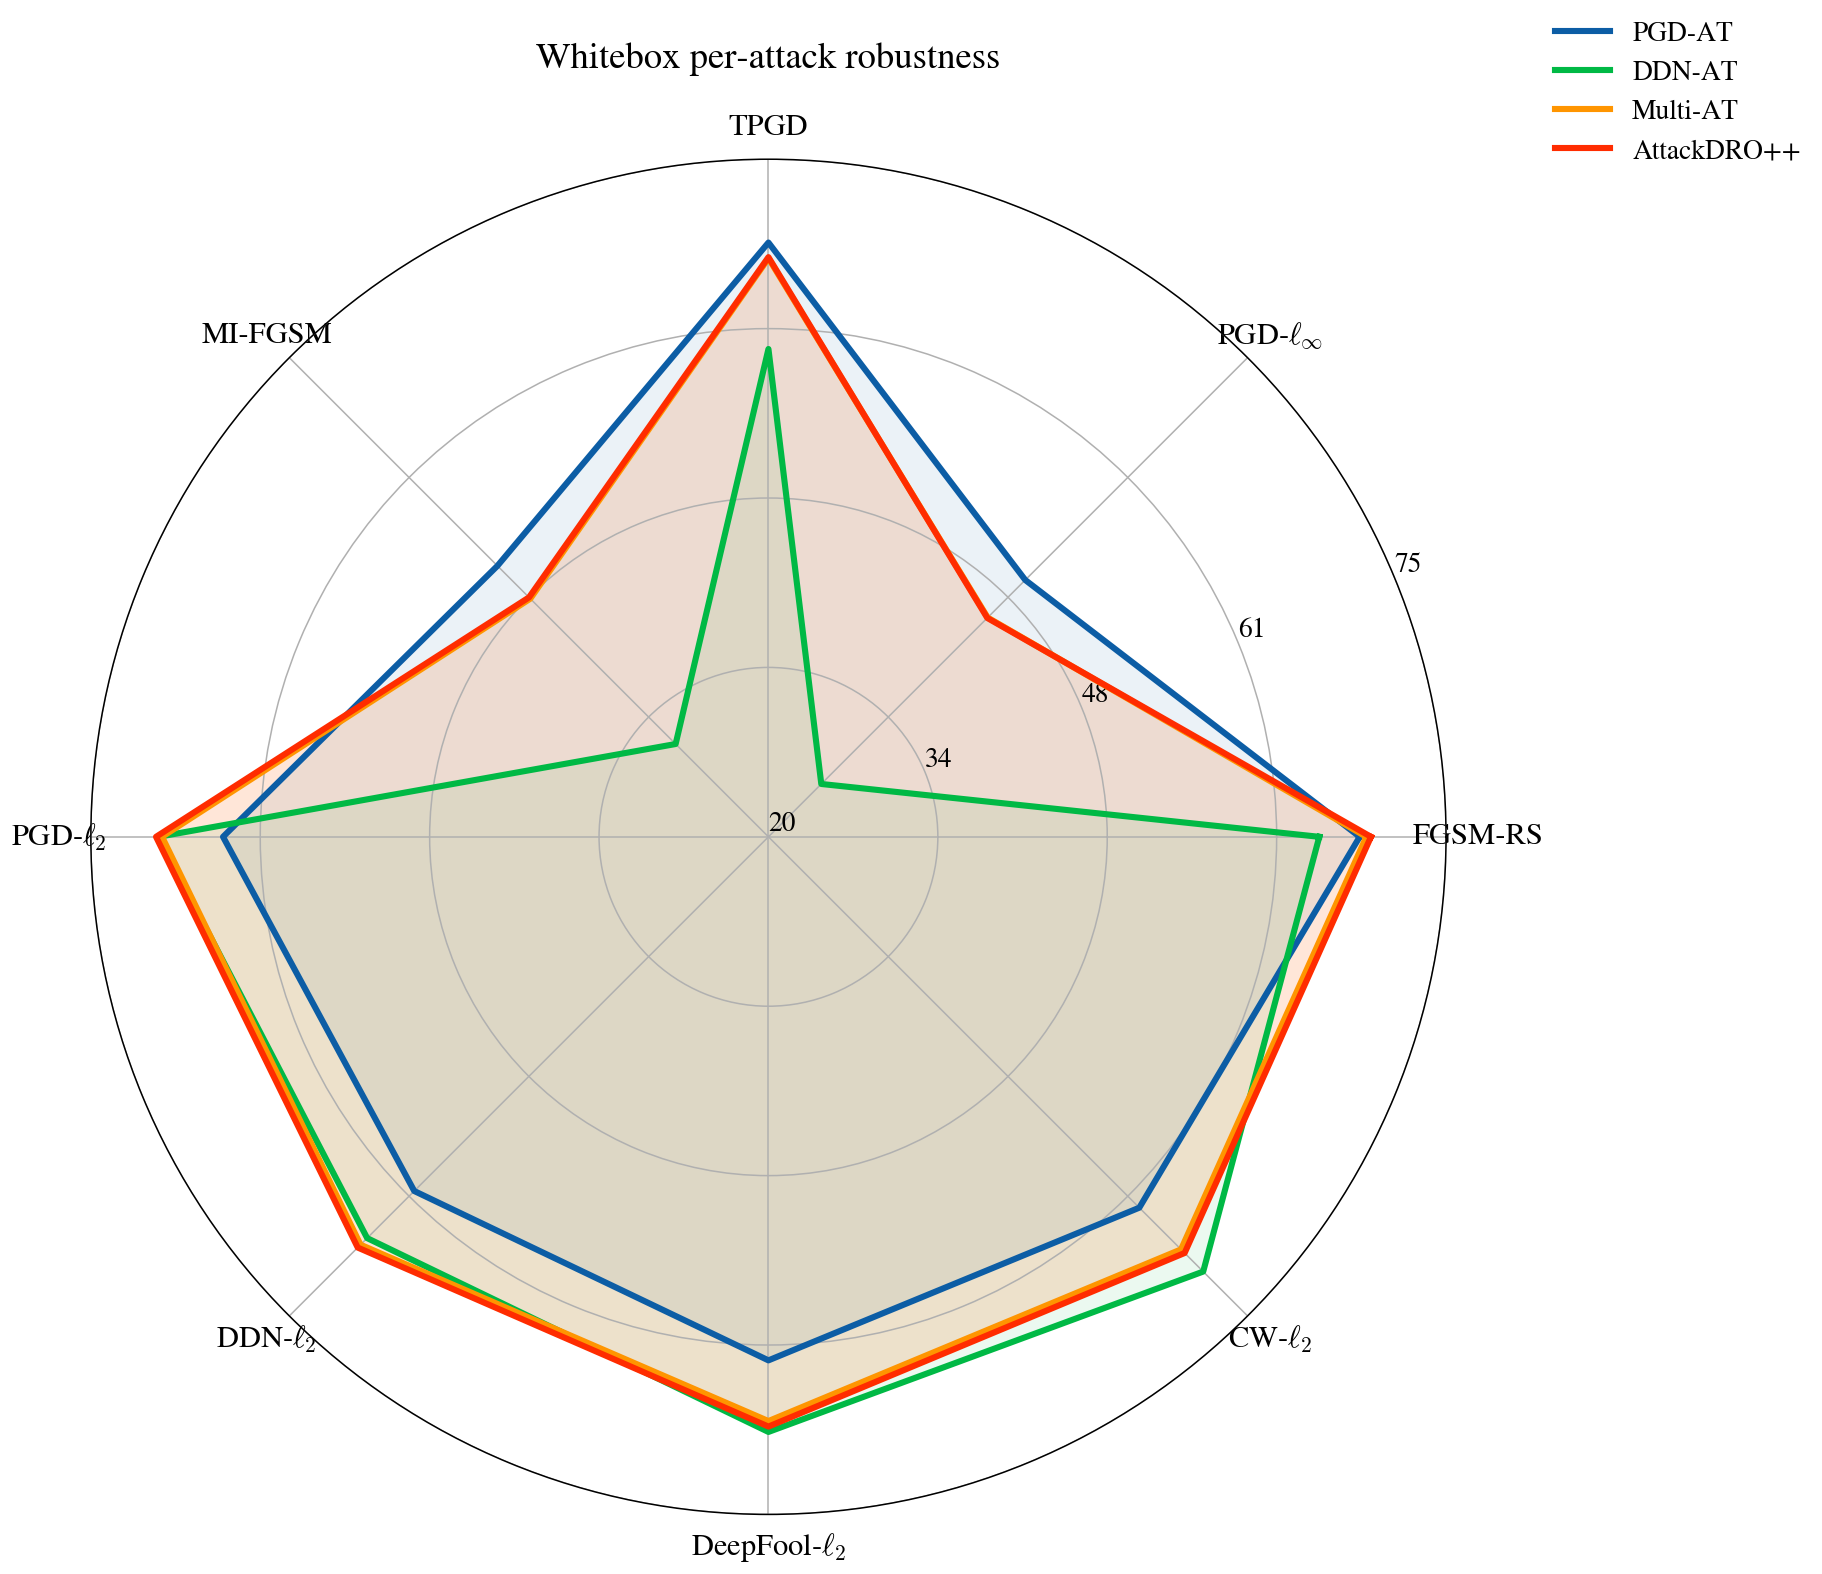
\includegraphics[width=0.78\linewidth]{figures/whitebox/whitebox_radar_per_attack_accuracy_n5.png}
\caption{Whitebox per-attack robustness profile averaged over five seeds. The radar plot compares PGD-AT, DDN-AT, Multi-AT, and AttackDRO++ (Ours) across the eight non-AutoAttack evaluation attacks. The shape of each curve highlights the specialization of the single-attack baselines and the more balanced profile of the multi-attack methods.}
\label{fig:ch6_whitebox_radar_per_attack_accuracy}
\end{figure}

\paragraph{Absolute per-class heatmaps with a shared scale.}
Before analyzing deltas, we first report the raw per-(class $\times$ attack) robust accuracy of each method. All four heatmaps use the same global color scale from 0\% to 100\%. This shared scale is important because it makes the maps visually comparable across methods: a darker cell always represents the same absolute robust accuracy, regardless of which method is being shown. 

\begin{figure}[H]
\centering
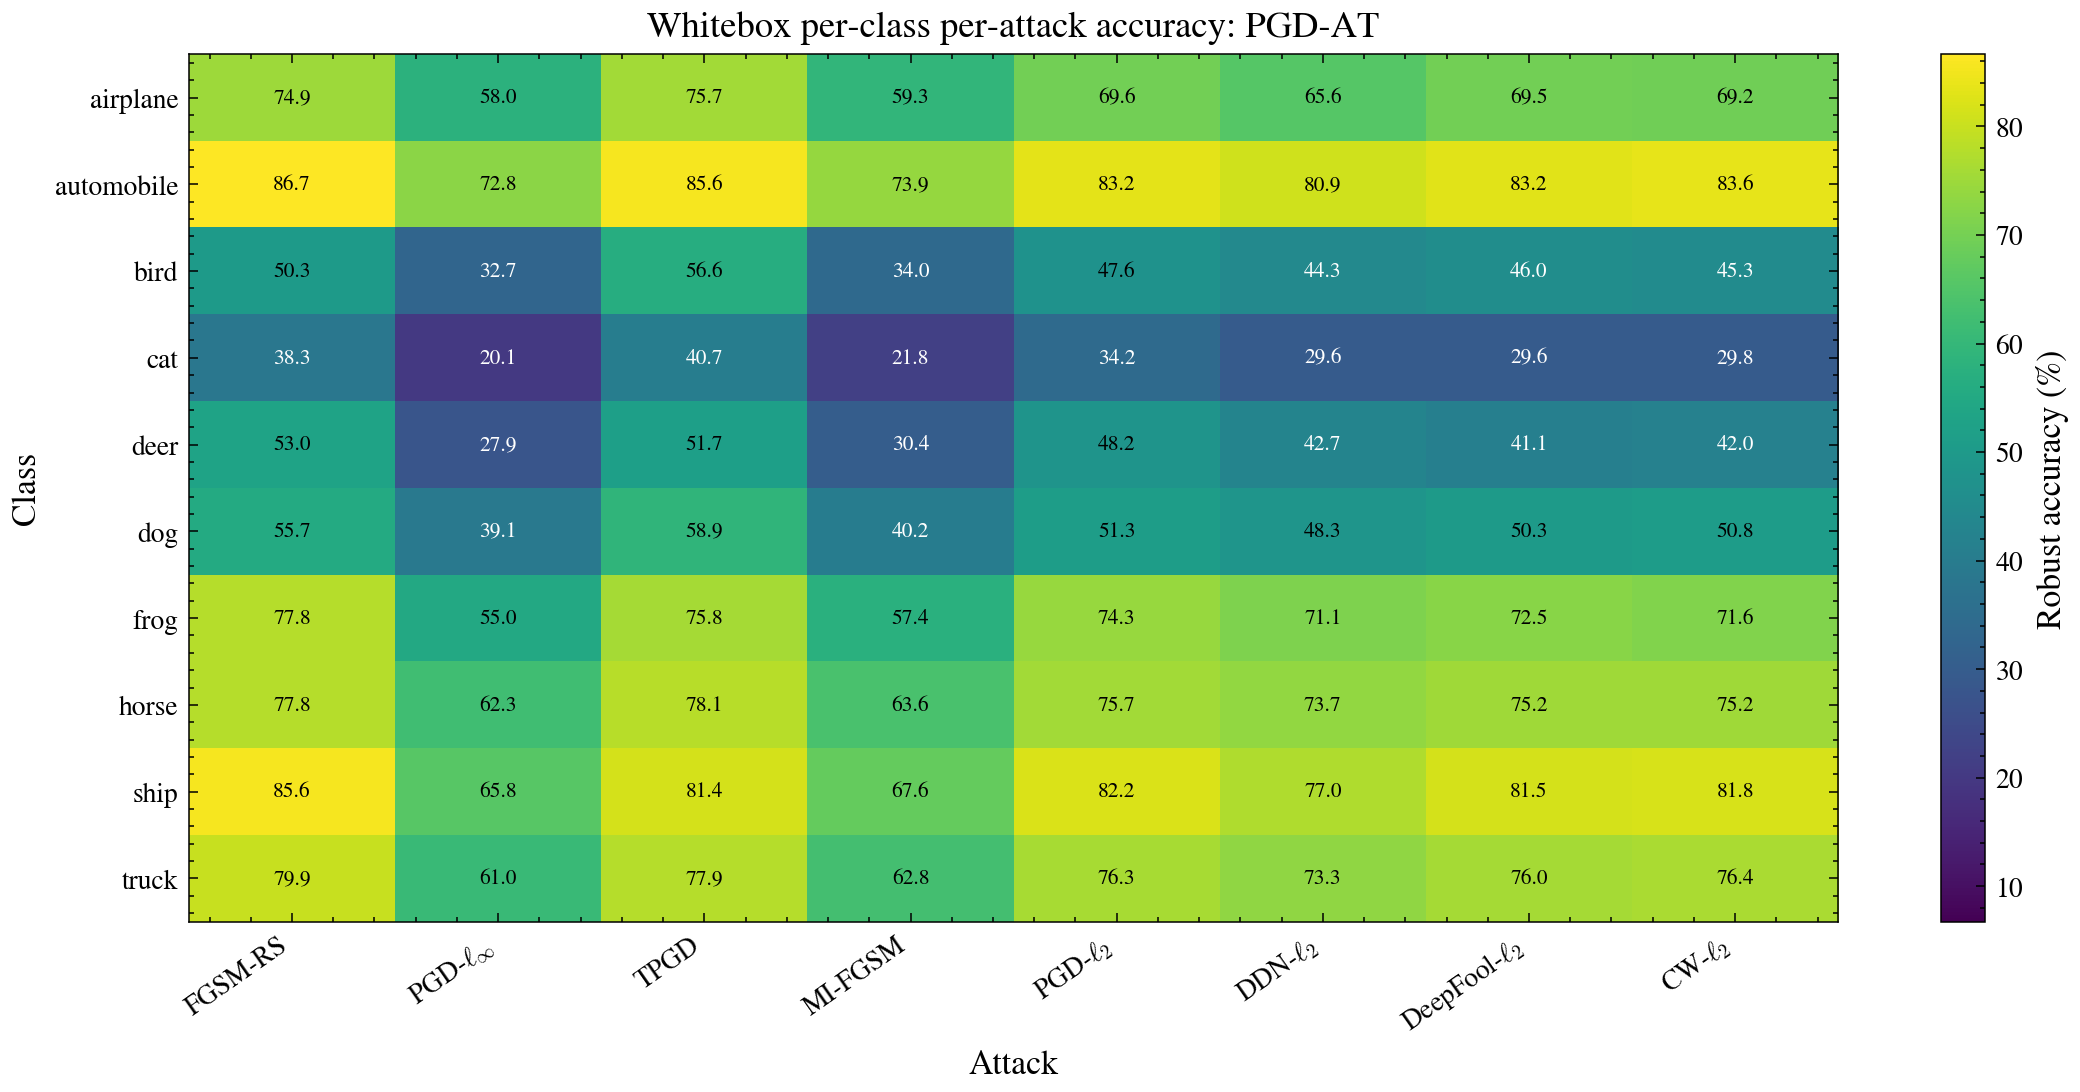
\includegraphics[width=\linewidth]{figures/whitebox/whitebox_per_class_attack_PGDAT_n5.png}
\caption{Absolute whitebox per-(class \(\times\) attack) robust accuracy
for PGD-AT. Cells report robust accuracy (\%).}
\label{fig:ch6_whitebox_abs_pgdat}
\end{figure}

\begin{figure}[H]
\centering
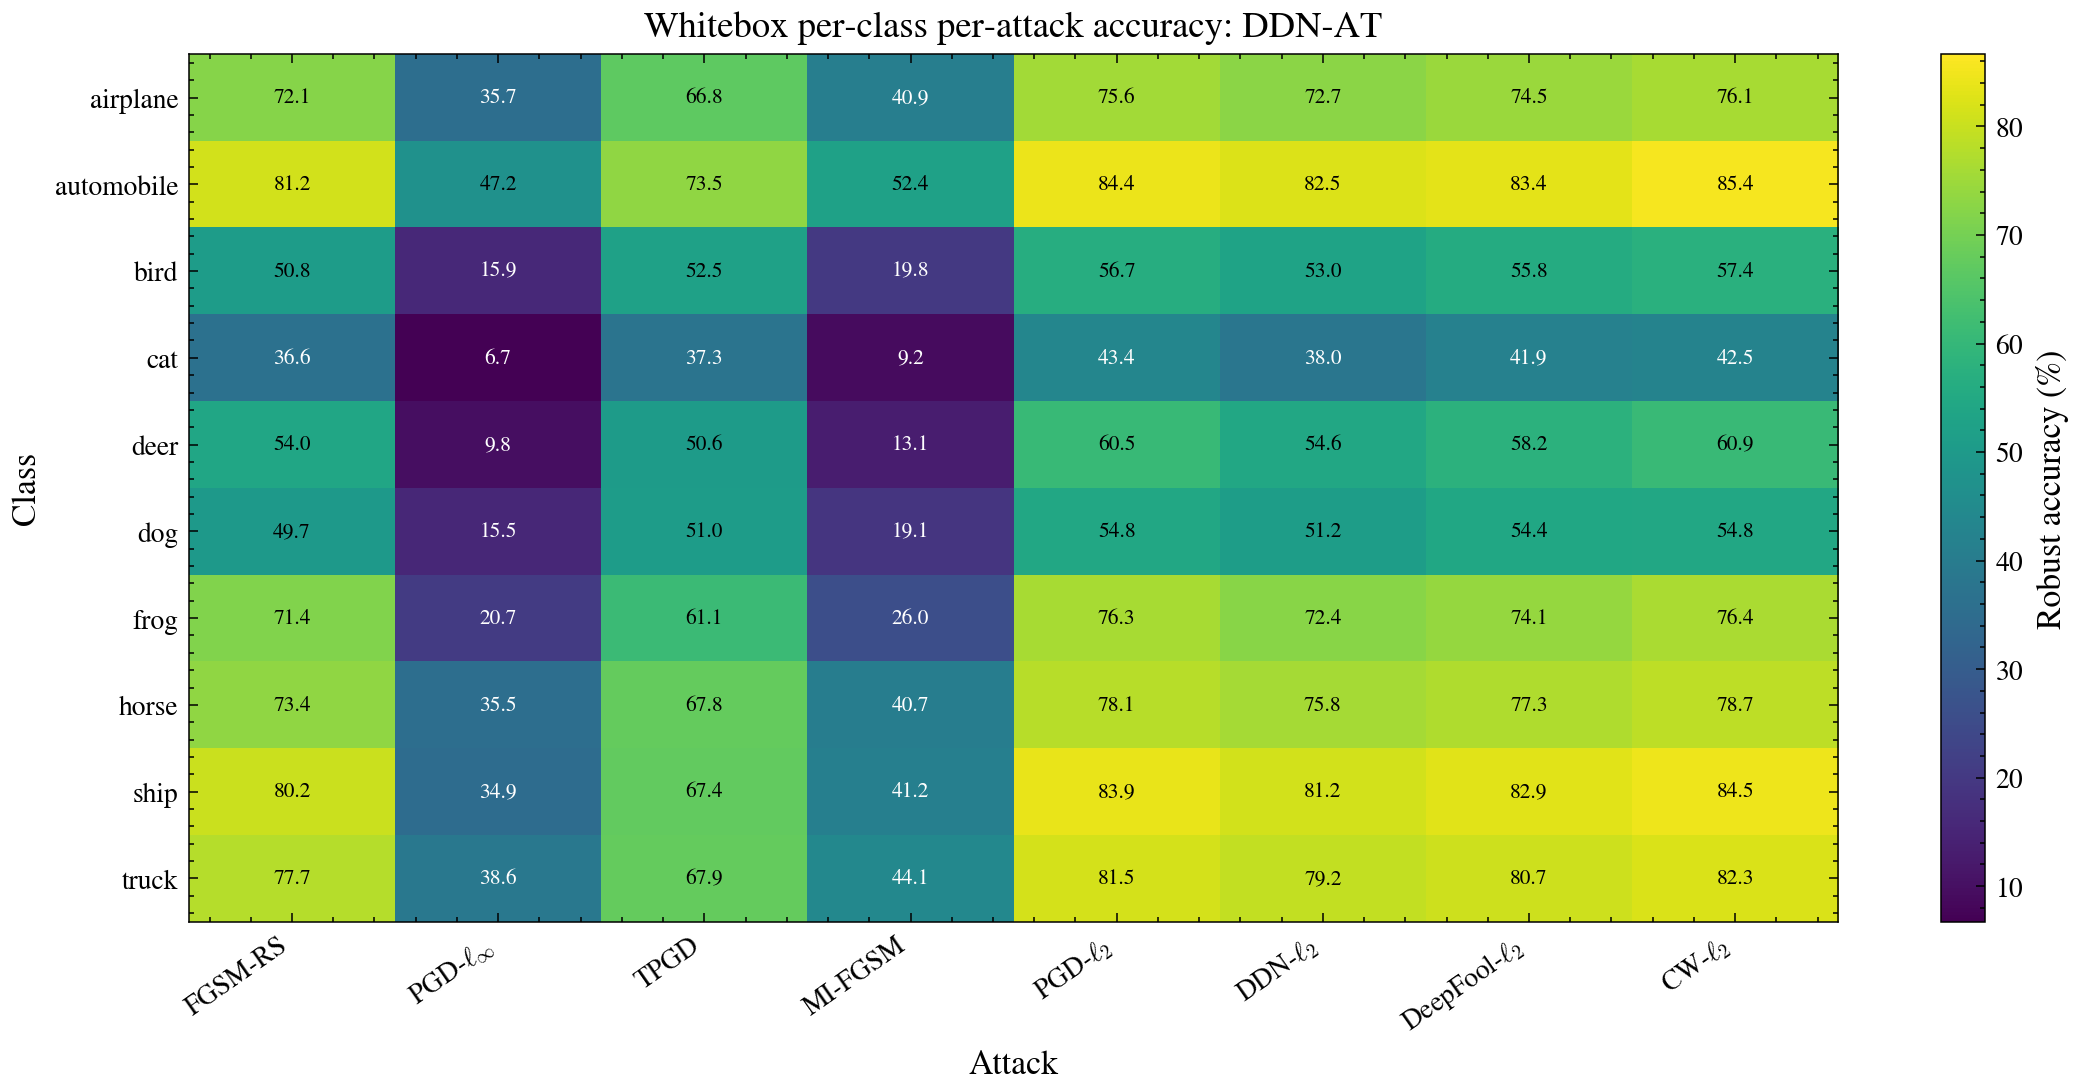
\includegraphics[width=\linewidth]{figures/whitebox/whitebox_per_class_attack_DDNAT_n5.png}
\caption{Absolute whitebox per-(class \(\times\) attack) robust accuracy
for DDN-AT. Cells report robust accuracy (\%).}
\label{fig:ch6_whitebox_abs_ddnat}
\end{figure}

\begin{figure}[H]
\centering
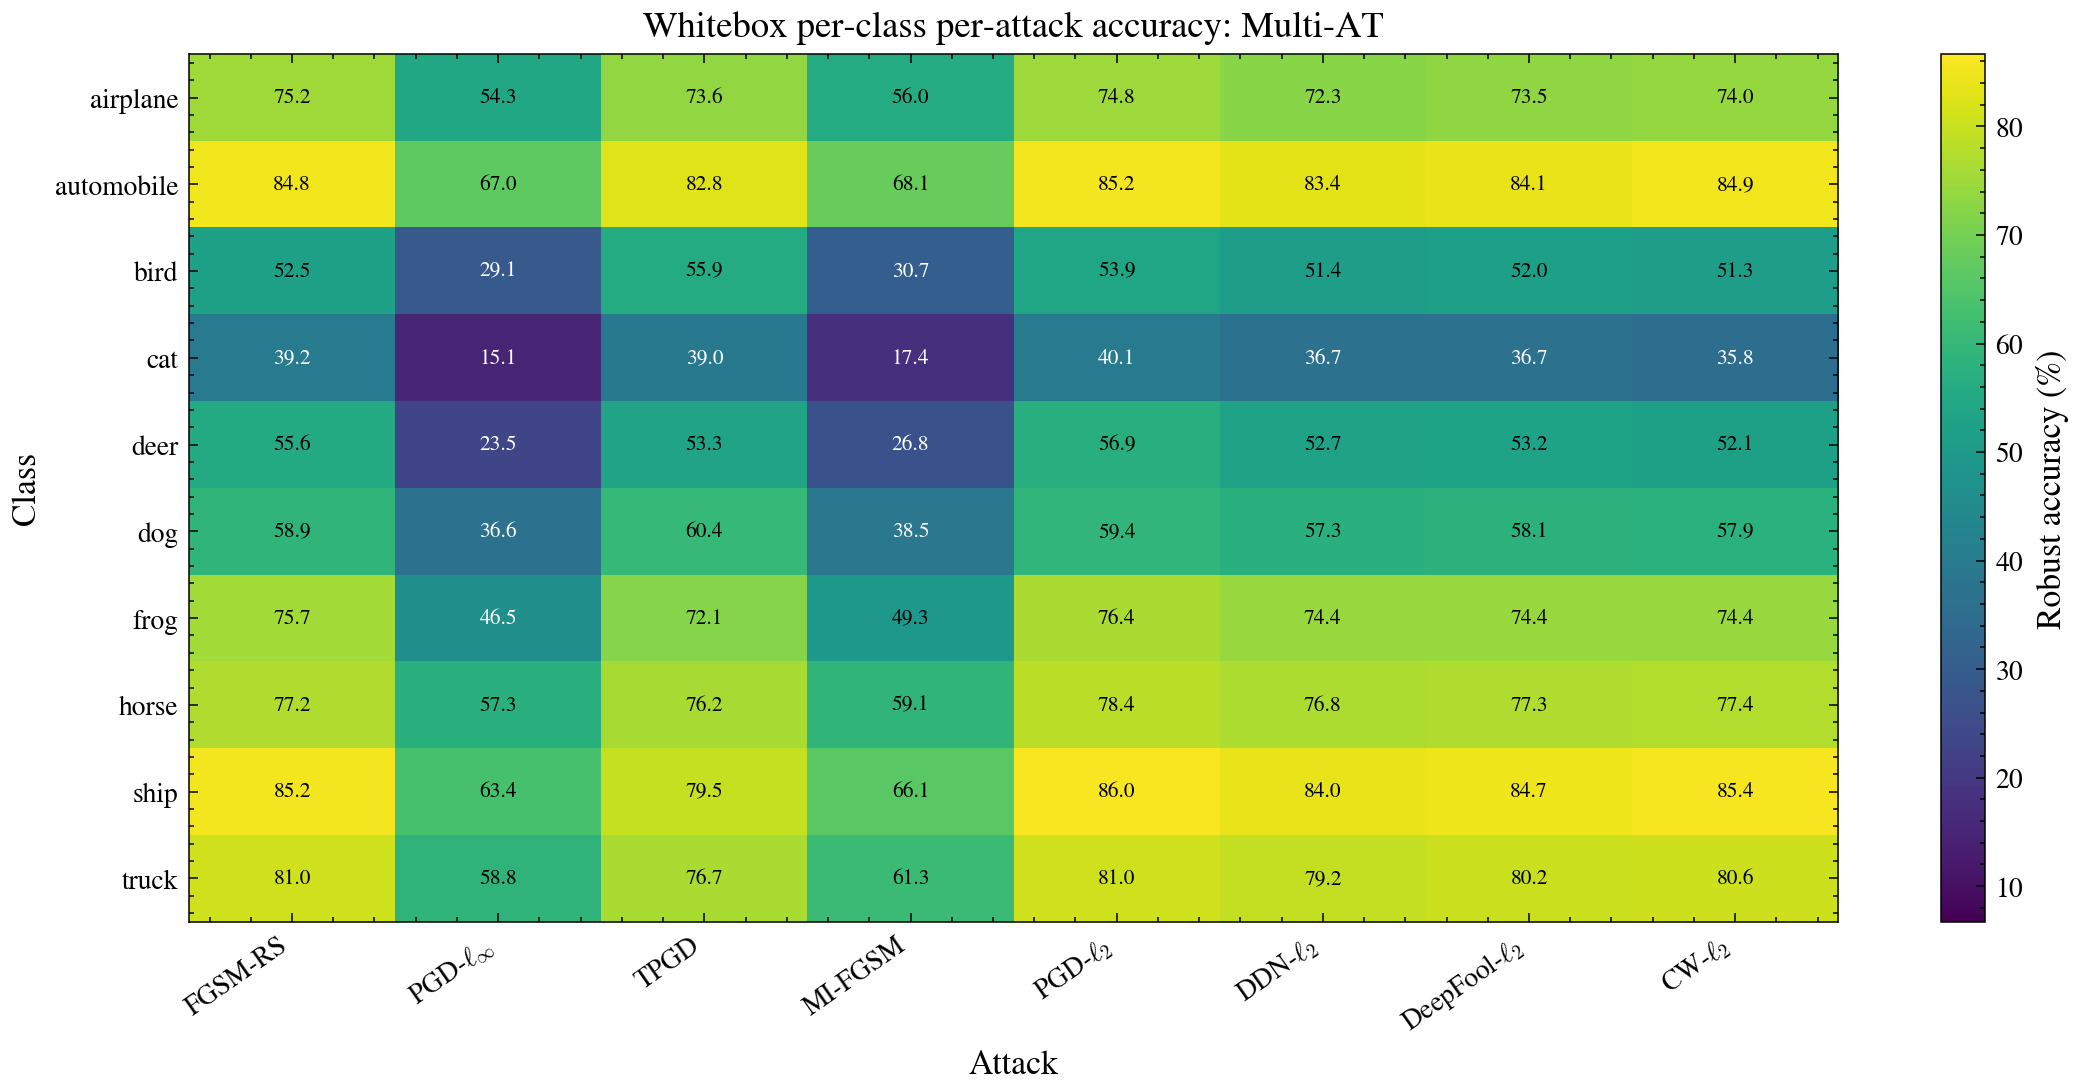
\includegraphics[width=\linewidth]{figures/whitebox/whitebox_per_class_attack_MultiAT_n5.png}
\caption{Absolute whitebox per-(class \(\times\) attack) robust accuracy
for Multi-AT. Cells report robust accuracy (\%).}
\label{fig:ch6_whitebox_abs_multiat}
\end{figure}

\begin{figure}[H]
\centering
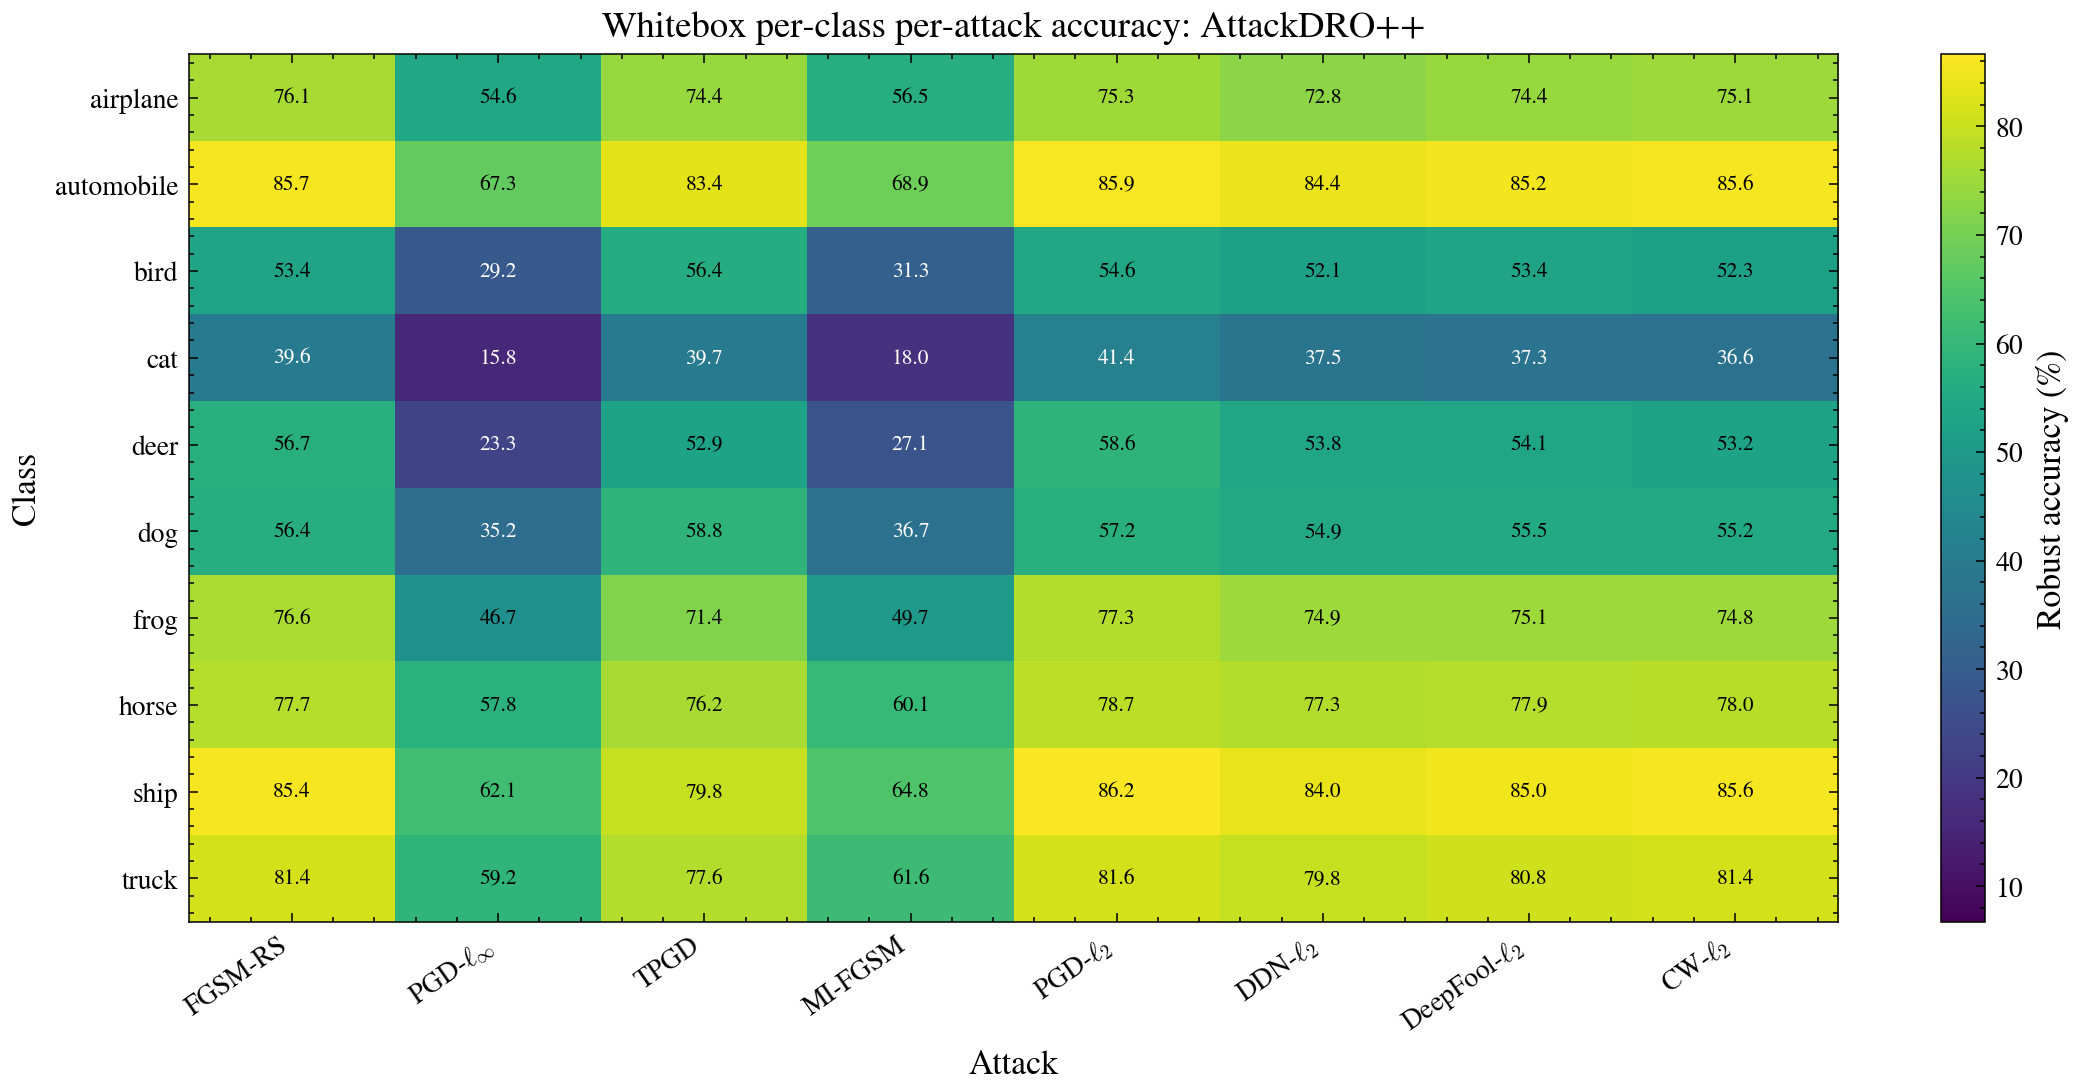
\includegraphics[width=\linewidth]{figures/whitebox/whitebox_per_class_attack_AttackDROpp_n5.png}
\caption{Absolute whitebox per-(class \(\times\) attack) robust accuracy
for AttackDRO++ (Ours). Cells report robust accuracy (\%).}
\label{fig:ch6_whitebox_abs_attackdropp}
\end{figure}
PGD-AT is stronger on several $\ell_\infty$ cells, while DDN-AT is more biased toward bounded $\ell_2$ attacks and visibly weaker on PGD-$\ell_\infty$ and MI-FGSM. Compared with the specialists, Multi-AT and AttackDRO++ show a more balanced cross-attack profile. AttackDRO++ largely preserves the Multi-AT structure while slightly lifting many cells, especially outside the hardest $\ell_\infty$ animal-class tail.

\subsection{Class-Level Gains and Persistent Difficulties}
\label{subsec:ch6_class_level_gains}

% TODO[Kiệt]:
% Goal:
% - Explain the main class-wise patterns without enumerating every class.
% Flow:
% - Identify broad high/low cells, then compare AttackDRO++ against Multi-AT and single-attack specialists.
% Include:
% - Reference `tab:ch6_whitebox_per_cell_summary` and the delta heatmaps.
% Avoid:
% - Unsupported causal claims about why individual CIFAR-10 classes are hard.
% Target length: 3-5 paragraphs.

Across all methods, the per-class robustness pattern is highly non-uniform. Classes such as \textit{automobile}, \textit{ship}, and \textit{truck} tend to remain easier under most attacks, while \textit{cat}, \textit{deer}, \textit{bird}, and \textit{dog} form the recurring hard tail. This pattern is consistent with the visual similarity and intra-class variation of CIFAR-10: animal classes often share local textures and backgrounds, so small adversarial perturbations can more easily move samples across nearby decision regions.

The hardest whitebox cells are concentrated in the $\ell_\infty$ iterative attacks. For AttackDRO++, the lowest cells are PGD-$\ell_\infty$ on \textit{cat} and \textit{deer}, followed by MI-FGSM on the same classes. This indicates that, even though AttackDRO++ improves the average multi-attack profile, the most difficult failure modes are still driven by strong $\ell_\infty$ optimization on semantically similar animal classes. In contrast, bounded $\ell_2$ attacks such as PGD-$\ell_2$, DDN-$\ell_2$, DeepFool-$\ell_2$, and CW-$\ell_2$ are generally less damaging for the proposed model than the strongest $\ell_\infty$ cells.

\paragraph{Attack-Class Delta Against Multi-AT Baseline}
Compared with Multi-AT, AttackDRO++ produces a broad but modest shift rather than a large change concentrated in a few cells. The mean per-cell gain is only $+0.281$ percentage points, but 67 out of 80 attack--class cells are positive.


\begin{figure}[H]
\centering
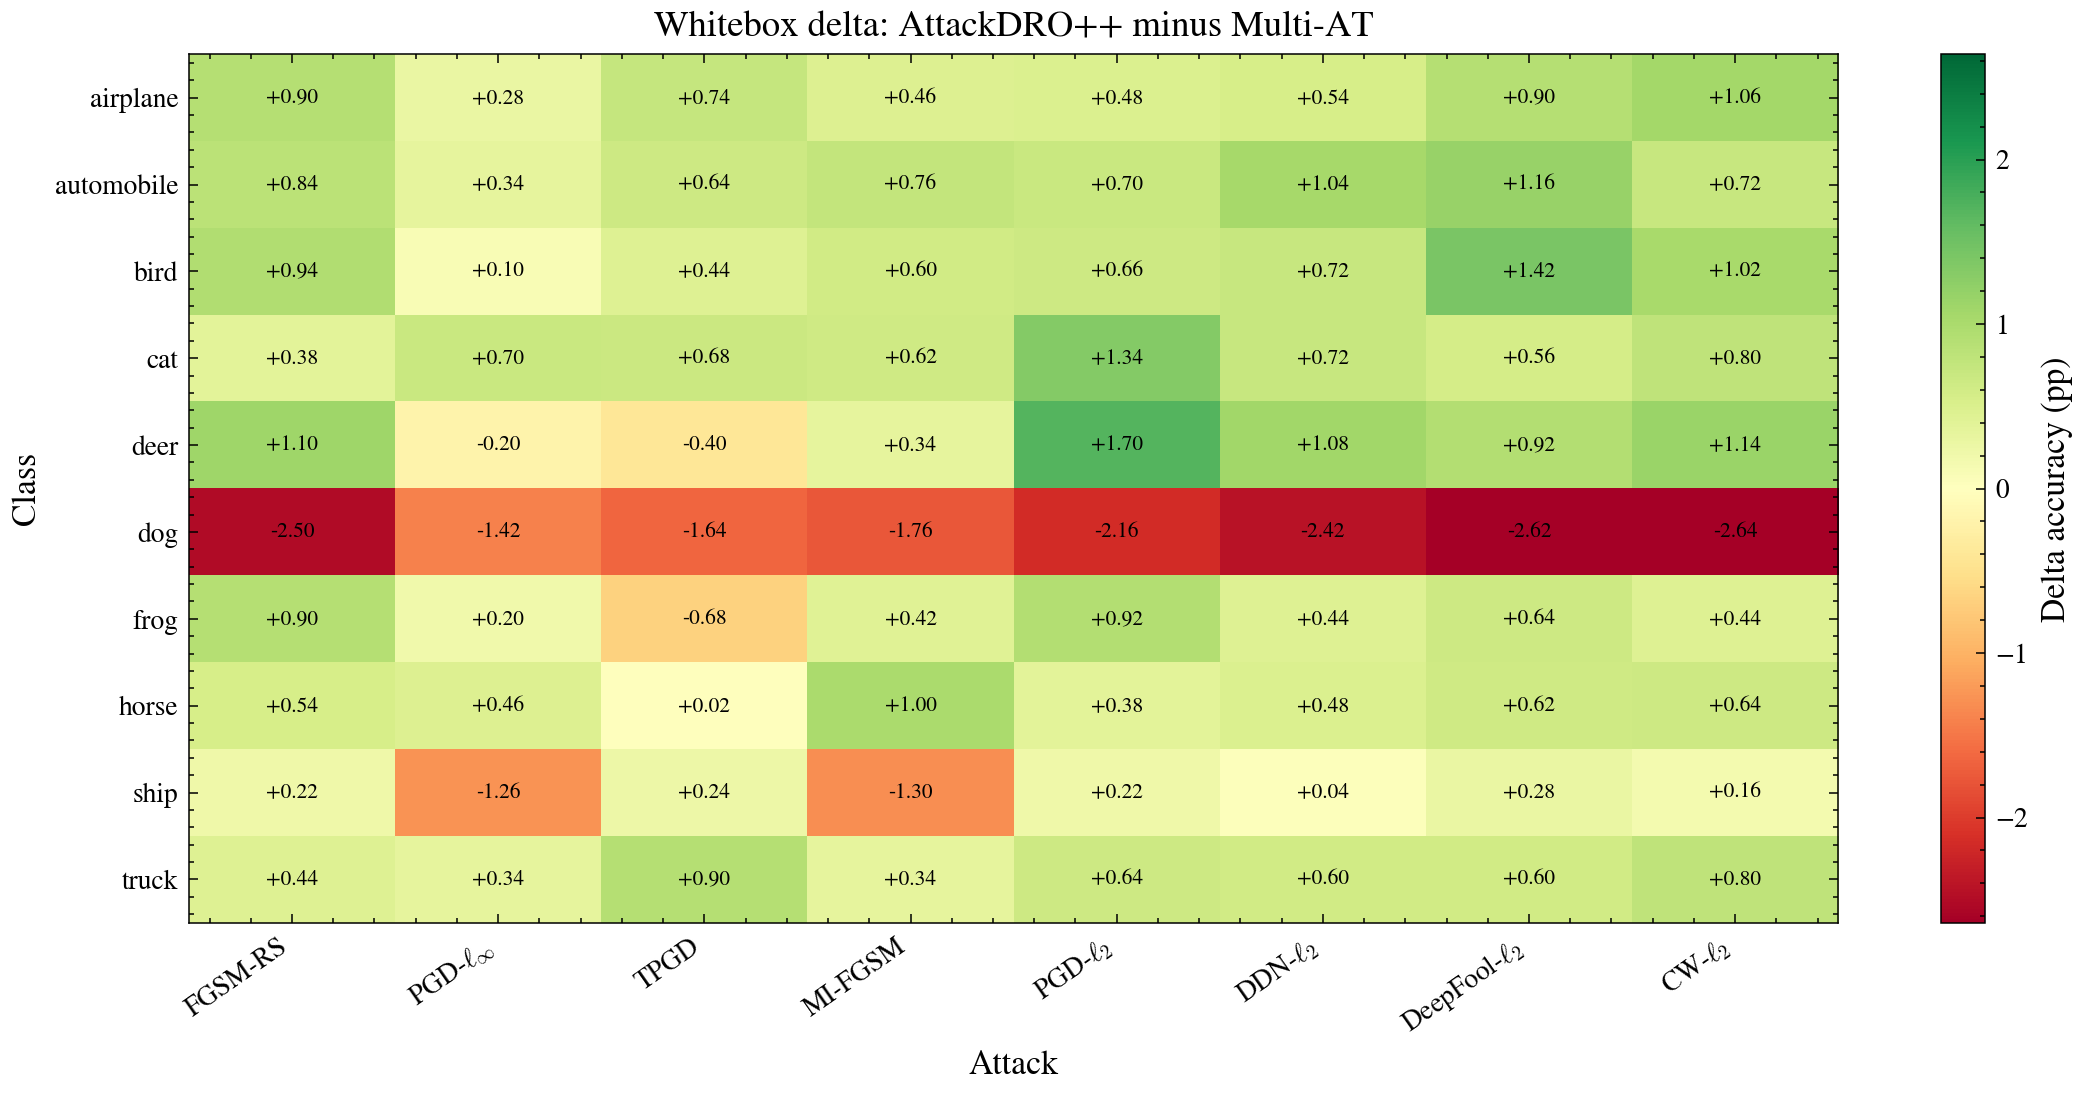
\includegraphics[width=\linewidth]{figures/whitebox/whitebox_delta_per_class_attack_AttackDROpp_vs_MultiAT_n5.png}
\caption{Whitebox per-(class $\times$ attack) delta of AttackDRO++ relative to Multi-AT. Each cell reports AttackDRO++ minus Multi-AT in percentage points, averaged over five seeds.}
\label{fig:ch6_whitebox_delta_vs_multiat}
\end{figure}

\paragraph{Attack-Class Delta Against Single-AT Baselines}

Table~\ref{tab:ch6_whitebox_per_cell_summary} summarizes the per-cell delta between AttackDRO++ and each baseline. The comparison against Multi-AT is the most important one because both methods train on the same source attacks and differ mainly in the group structure used for optimization. AttackDRO++ improves 67/80 cells over Multi-AT, with a mean gain of $+0.281$ percentage points and a bottom-10 lift of $+0.282$ percentage points. The gains are small, but they are widespread, which supports the interpretation that cluster-based DRO acts as a stabilizing refinement over uniform multi-attack training.

\begin{table}[H]
\centering
\caption{Per-(class $\times$ attack) whitebox comparison of AttackDRO++ against each baseline. $\Delta$ is computed as AttackDRO++ minus the baseline. Positive cells count the number of attack--class cells where $\Delta>0$ out of 80 total cells.}
\label{tab:ch6_whitebox_per_cell_summary}
\footnotesize
\setlength{\tabcolsep}{4.5pt}
\renewcommand{\arraystretch}{1.18}
\begin{tabular}{lccccc}
\toprule
Baseline
& Positive cells
& Mean
& Significant cells
& Bottom-10
& Main pattern \\
& $(\Delta>0)$
& $\Delta$ (pp)
& AttackDRO++ / Baseline
& lift (pp)
& \\
\midrule
Multi-AT
& 67/80
& $+0.281$
& 0 / 2
& $+0.282$
& Balanced refinement \\
PGD-AT
& 47/80
& $+1.782$
& 40 / 19
& $+0.726$
& Gains mainly on $\ell_2$ cells \\
DDN-AT
& 62/80
& $+5.781$
& 44 / 5
& $+15.710$
& Gains mainly on $\ell_\infty$ cells \\
\bottomrule
\end{tabular}

\end{table}

\begin{figure}[H]
\centering
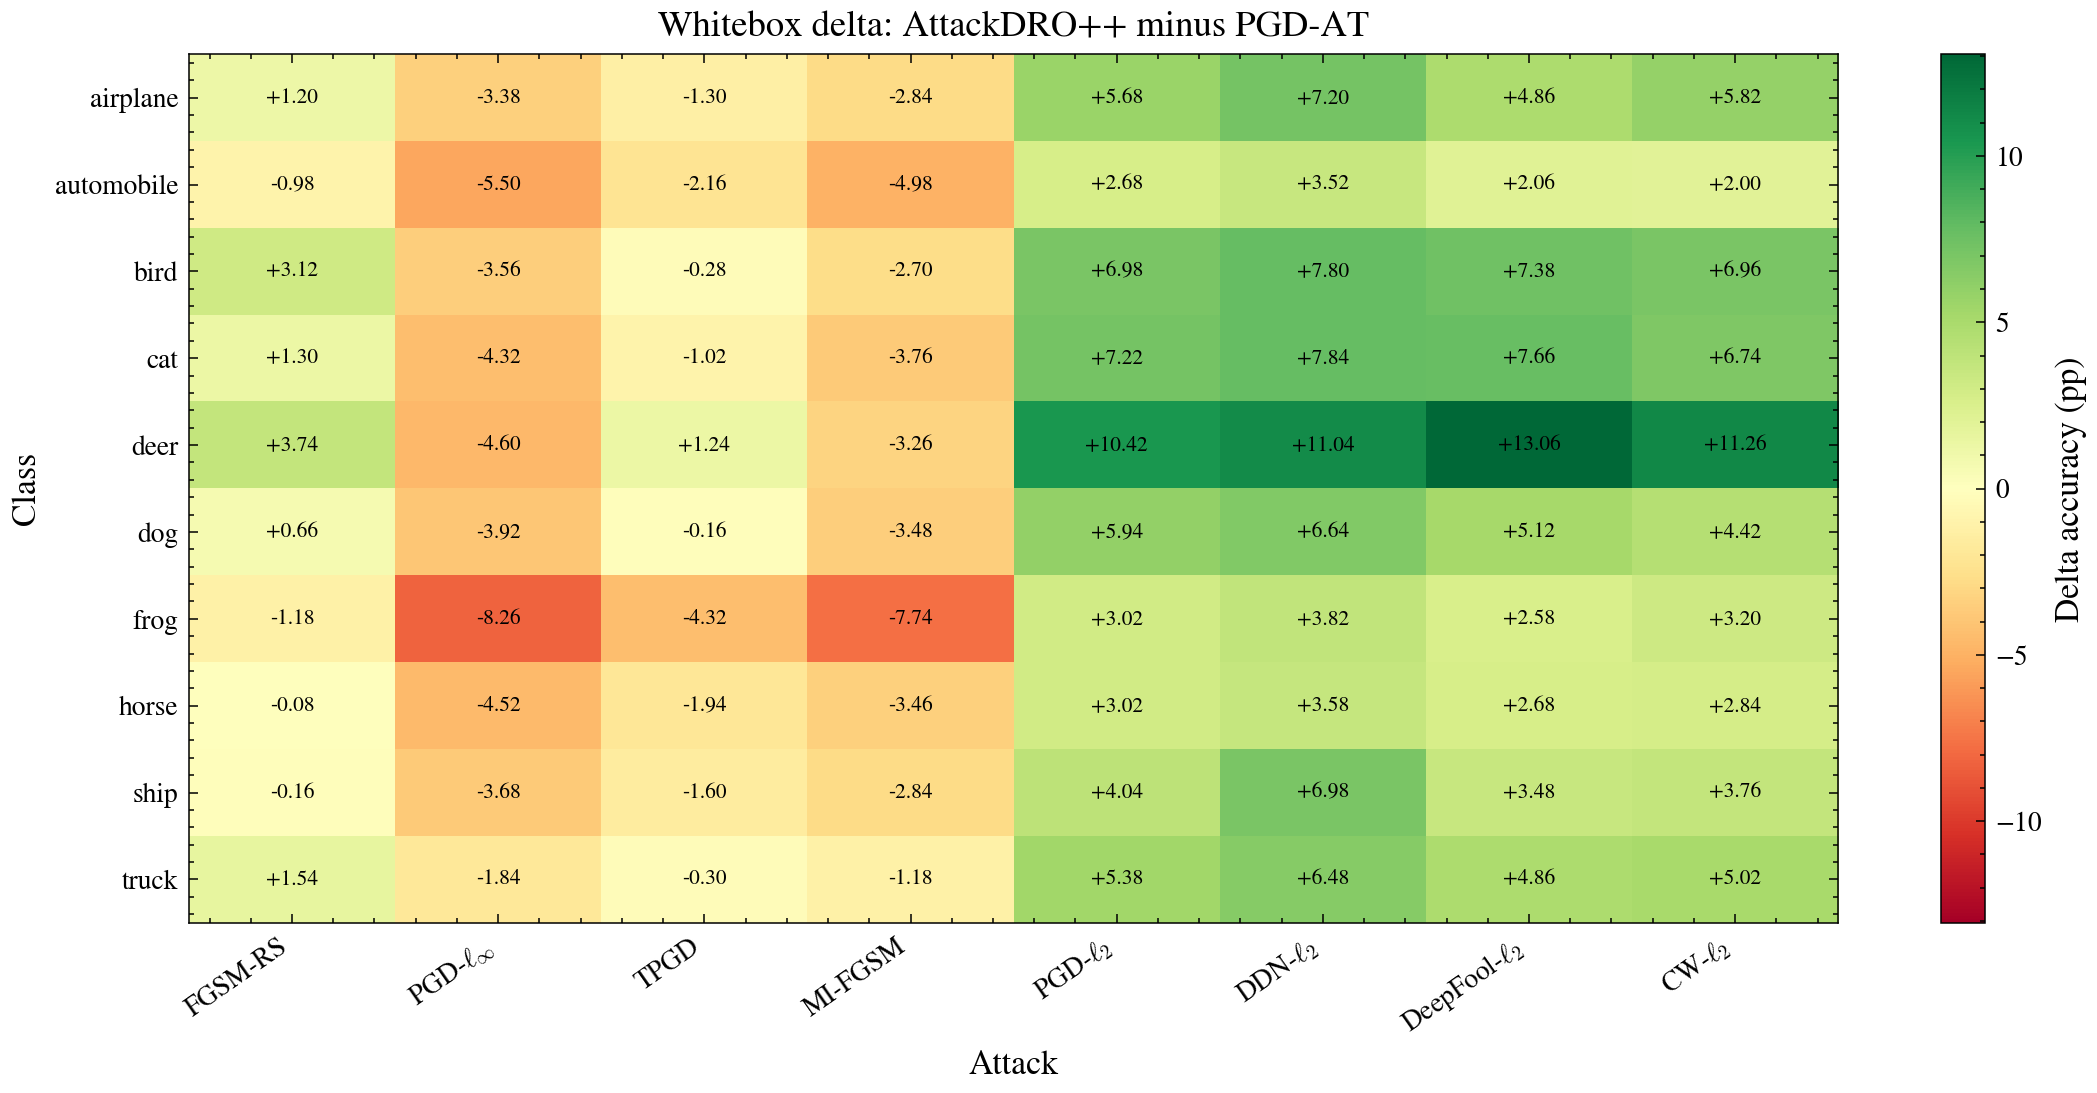
\includegraphics[width=\linewidth]{figures/whitebox/whitebox_delta_per_class_attack_AttackDROpp_vs_PGDAT_n5.png}
\caption{Whitebox per-(class $\times$ attack) delta of AttackDRO++ (Ours) relative to PGD-AT. Positive cells indicate where AttackDRO++ (Ours) improves over the PGD-$\ell_\infty$ specialist. Gains are concentrated mainly on bounded $\ell_2$ attacks, while PGD-AT remains stronger on several $\ell_\infty$ iterative cells.}
\label{fig:ch6_whitebox_delta_vs_pgdat}
\end{figure}

\begin{figure}[H]
\centering
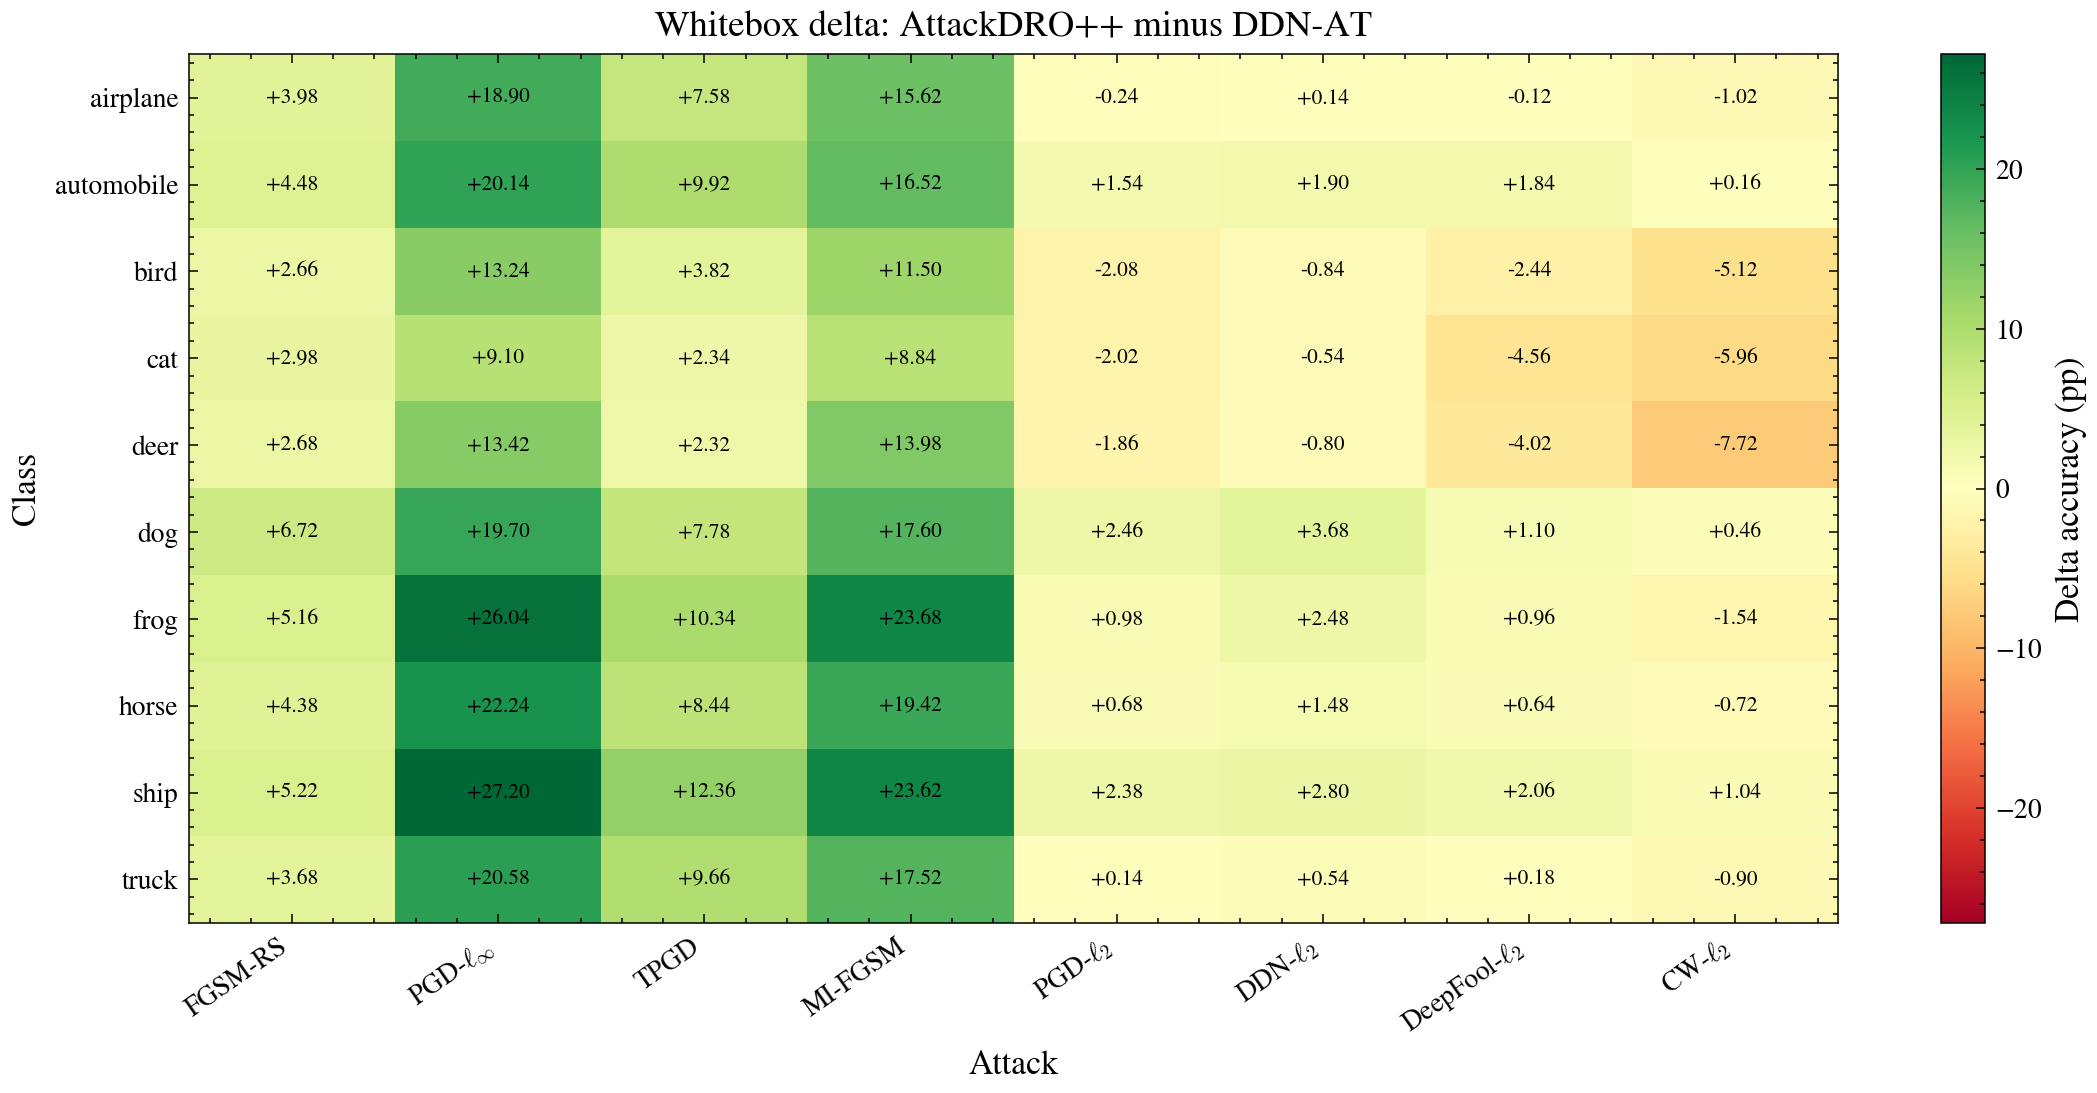
\includegraphics[width=\linewidth]{figures/whitebox/whitebox_delta_per_class_attack_AttackDROpp_vs_DDNAT_n5.png}
\caption{Whitebox per-(class $\times$ attack) delta of AttackDRO++ (Ours) relative to DDN-AT. The large positive cells under PGD-$\ell_\infty$ and MI-FGSM show that AttackDRO++ (Ours) substantially corrects the $\ell_\infty$ weakness of the DDN-$\ell_2$ specialist, while several negative cells remain on DDN-AT's preferred $\ell_2$ family.}
\label{fig:ch6_whitebox_delta_vs_ddnat}
\end{figure}

The comparison against PGD-AT shows the expected specialist trade-off. AttackDRO++ is positive in 47/80 cells and has a mean gain of $+1.782$ percentage points, but the gains and losses are not uniformly distributed. The largest improvements occur on bounded $\ell_2$ attacks, especially DeepFool-$\ell_2$, CW-$\ell_2$, DDN-$\ell_2$, and PGD-$\ell_2$ on hard animal classes such as \textit{deer}, \textit{cat}, and \textit{bird}. For example, the largest gains over PGD-AT appear on DeepFool-$\ell_2$ for \textit{deer} ($+13.06$ pp), CW-$\ell_2$ for \textit{deer} ($+11.26$ pp), and DDN-$\ell_2$ for \textit{deer} ($+11.04$ pp). Conversely, PGD-AT remains stronger on several $\ell_\infty$ cells, particularly PGD-$\ell_\infty$ and MI-FGSM for \textit{frog}, \textit{automobile}, \textit{horse}, and \textit{cat}. This confirms that PGD-AT is not weak in absolute terms; rather, it is specialized toward the $\ell_\infty$ geometry used during training.

The comparison against DDN-AT is even more asymmetric. AttackDRO++ improves 62/80 cells and gains $+5.781$ percentage points on average, with a large $+15.710$ percentage-point improvement on the bottom-10 cells. The largest improvements occur under $\ell_\infty$ attacks: PGD-$\ell_\infty$ on \textit{ship} ($+27.20$ pp), PGD-$\ell_\infty$ on \textit{frog} ($+26.04$ pp), MI-FGSM on \textit{frog} ($+23.68$ pp), and MI-FGSM on \textit{ship} ($+23.62$ pp). These large deltas show that DDN-AT develops a strong $\ell_2$ bias and leaves many $\ell_\infty$ attack--class cells under-protected. At the same time, DDN-AT remains stronger on some $\ell_2$ boundary/optimization cells, especially CW-$\ell_2$ and DeepFool-$\ell_2$ for \textit{deer}, \textit{cat}, and \textit{bird}. Thus, AttackDRO++ improves cross-attack balance but does not completely dominate the strongest single-norm specialist on its preferred family.

\paragraph{Attack-family interpretation.}

% TODO[Kiệt]:
% Goal:
% - Explain whether gains are balanced across attack families.
% Flow:
% - Compare source attacks, held-out `\ell_\infty`, and held-out `\ell_2` patterns.
% Include:
% - Reference the radar delta figure if kept in the main flow.
% Avoid:
% - Using metric shorthand in headings or unexplained captions.
% Target length: 2-4 paragraphs.

The attack-wise deltas make the specialization effect clear. Relative to PGD-AT, AttackDRO++ loses on PGD-$\ell_\infty$ and MI-FGSM on average, but gains strongly on the bounded $\ell_2$ attacks. Relative to DDN-AT, the pattern reverses: AttackDRO++ gains substantially on PGD-$\ell_\infty$, MI-FGSM, TPGD, and FGSM-RS, while being slightly weaker on CW-$\ell_2$ and DeepFool-$\ell_2$. 
The Multi-AT comparison is more balanced: most attack averages are positive, but the magnitudes are below one percentage point.

\begin{figure}[H]
\centering
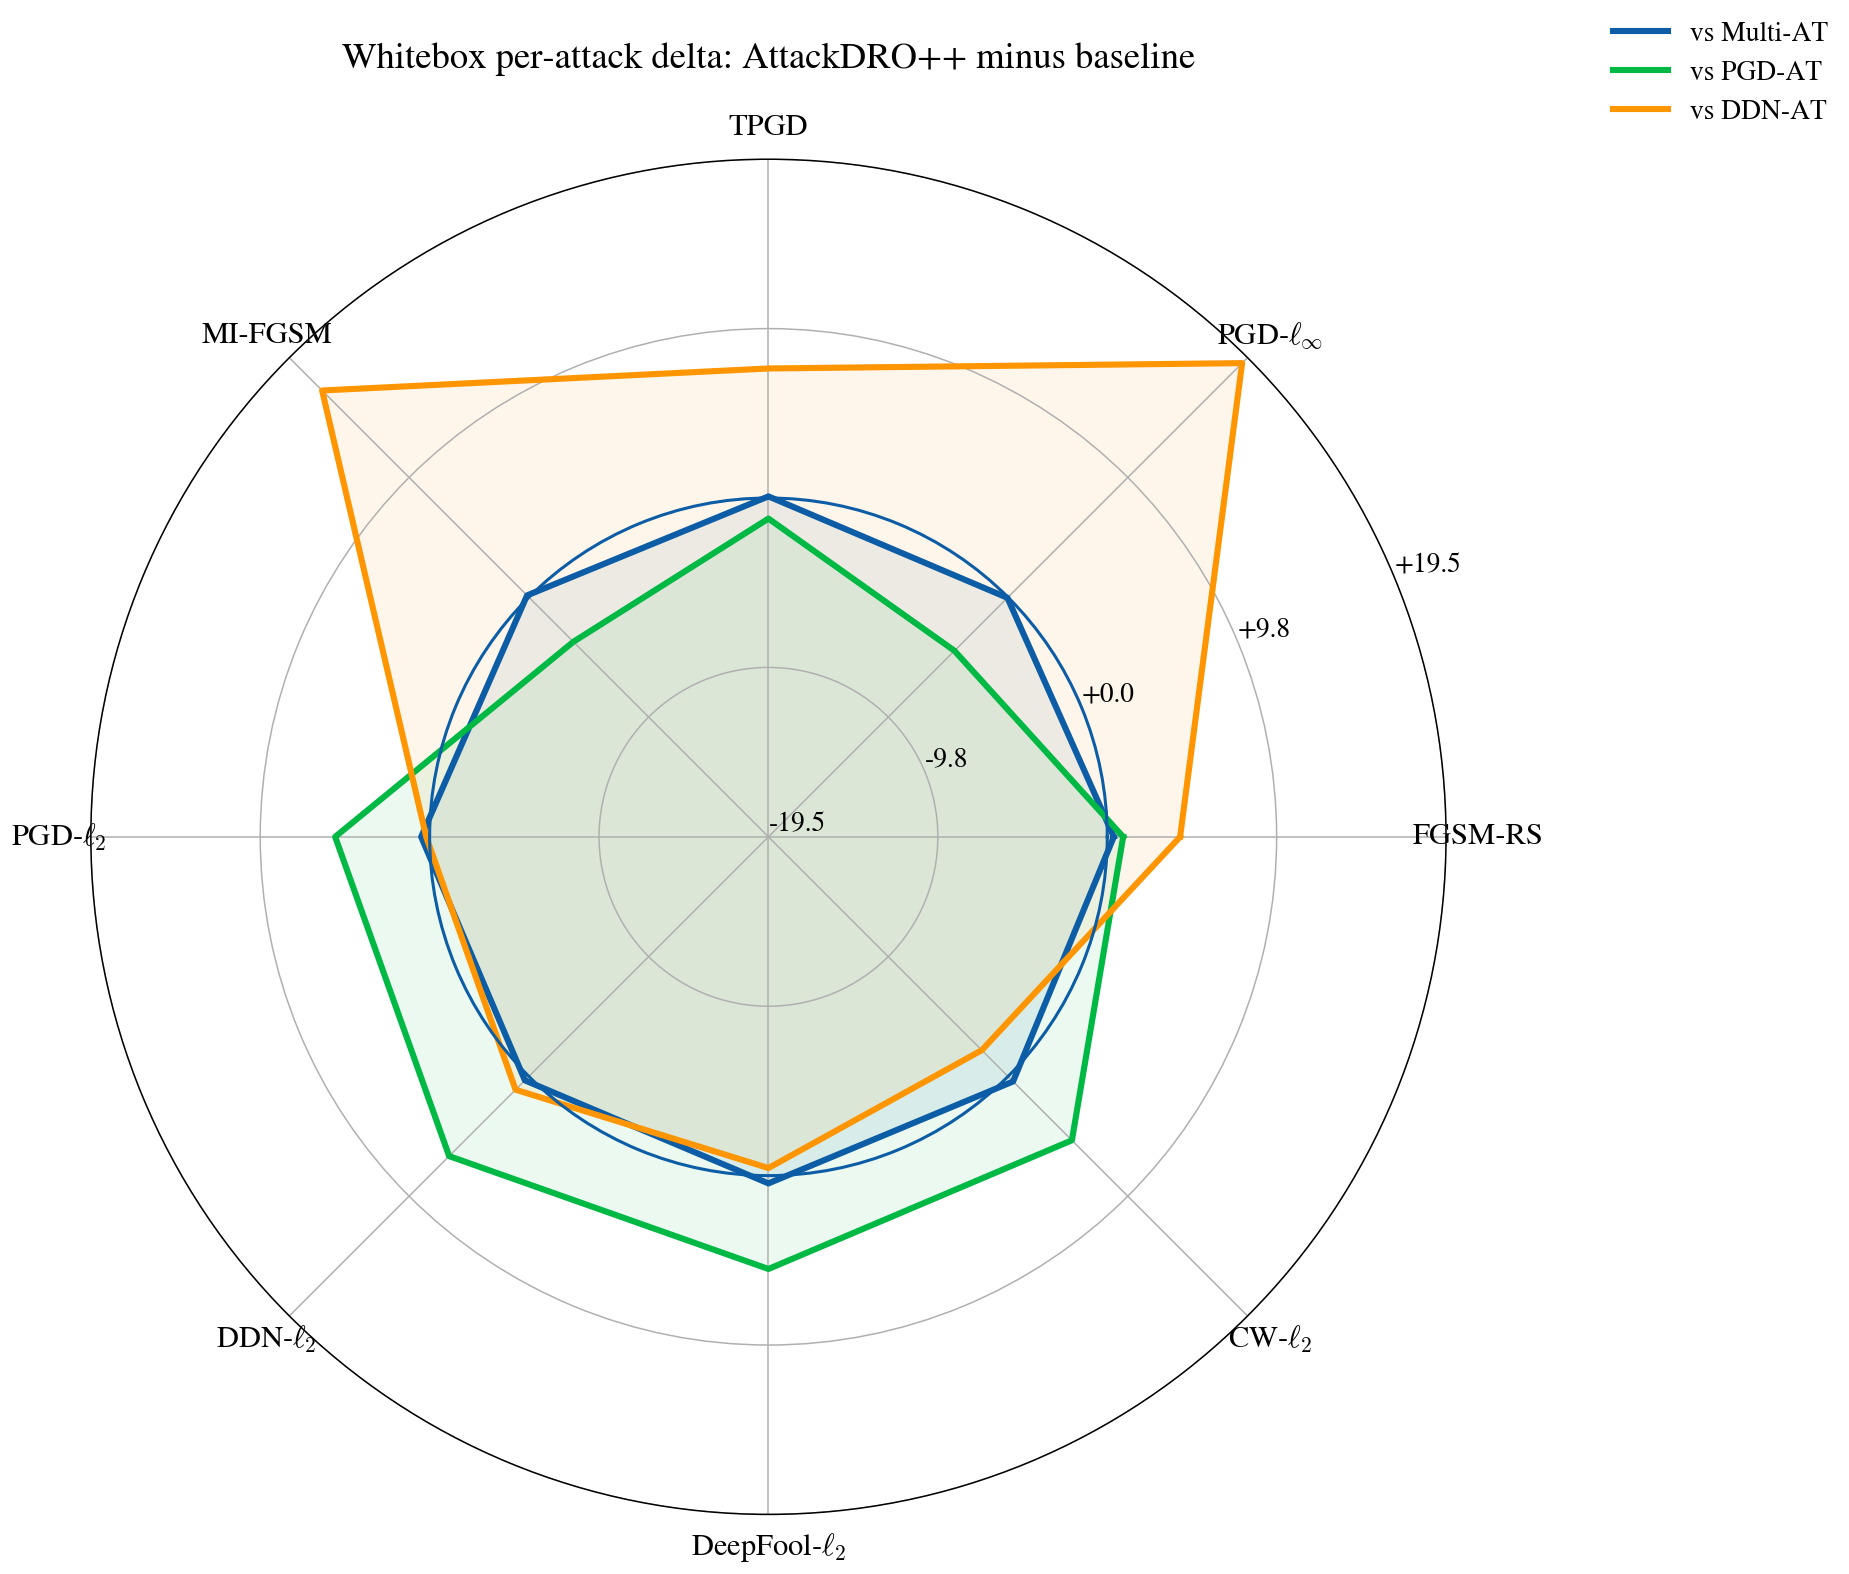
\includegraphics[width=\linewidth]{figures/whitebox/whitebox_radar_attackdropp_delta_vs_baselines_n5.png}
\caption{Attack-wise whitebox delta of AttackDRO++ relative to the three baselines.}
\label{fig:ch6_whitebox_radar_delta_vs_baselines}
\end{figure}
\vspace{-0.5cm}
This result supports the main claim of the chapter. AttackDRO++ should not be interpreted as a replacement for a single specialist when the deployment threat model is known exactly. Instead, it is a cross-attack robustness method: it sacrifices some of the peak strength of a specialist in exchange for a more even robustness profile across attacks and classes. 

\subsection{Tail-Class Robustness: Do the Weakest Cells Improve?}
\label{subsec:ch6_tail_class_robustness}

% TODO[Kiệt]:
% Goal:
% - Explain whether AttackDRO++ improves difficult tail cells, not only average cells.
% Flow:
% - Define Bottom-K locally or point to an earlier definition, then interpret the lift figure.
% Include:
% - Reference `fig:ch6_whitebox_bottomk_lift` if it remains in the main flow.
% Avoid:
% - Leaving `Bottom-K` as undefined shorthand.
% Target length: 2-3 paragraphs.

We next examine the weakest attack--class cells for each baseline, using
\(K \in \{5,10,20\}\). These cells capture localized failure modes that can be
hidden by mean accuracy. For Multi-AT, the weakest cells are mainly strong
\(\ell_\infty\) attacks, especially PGD-$\ell_\infty$ and MI-FGSM, on hard animal
classes such as \textit{cat}, \textit{deer}, and \textit{bird}. AttackDRO++
improves this tail only slightly: the bottom-10 lift is \(+0.282\) pp. Although
small, this shows that the average gain over Multi-AT is not obtained by
sacrificing its weakest cells.

\begin{figure}[H]
\centering
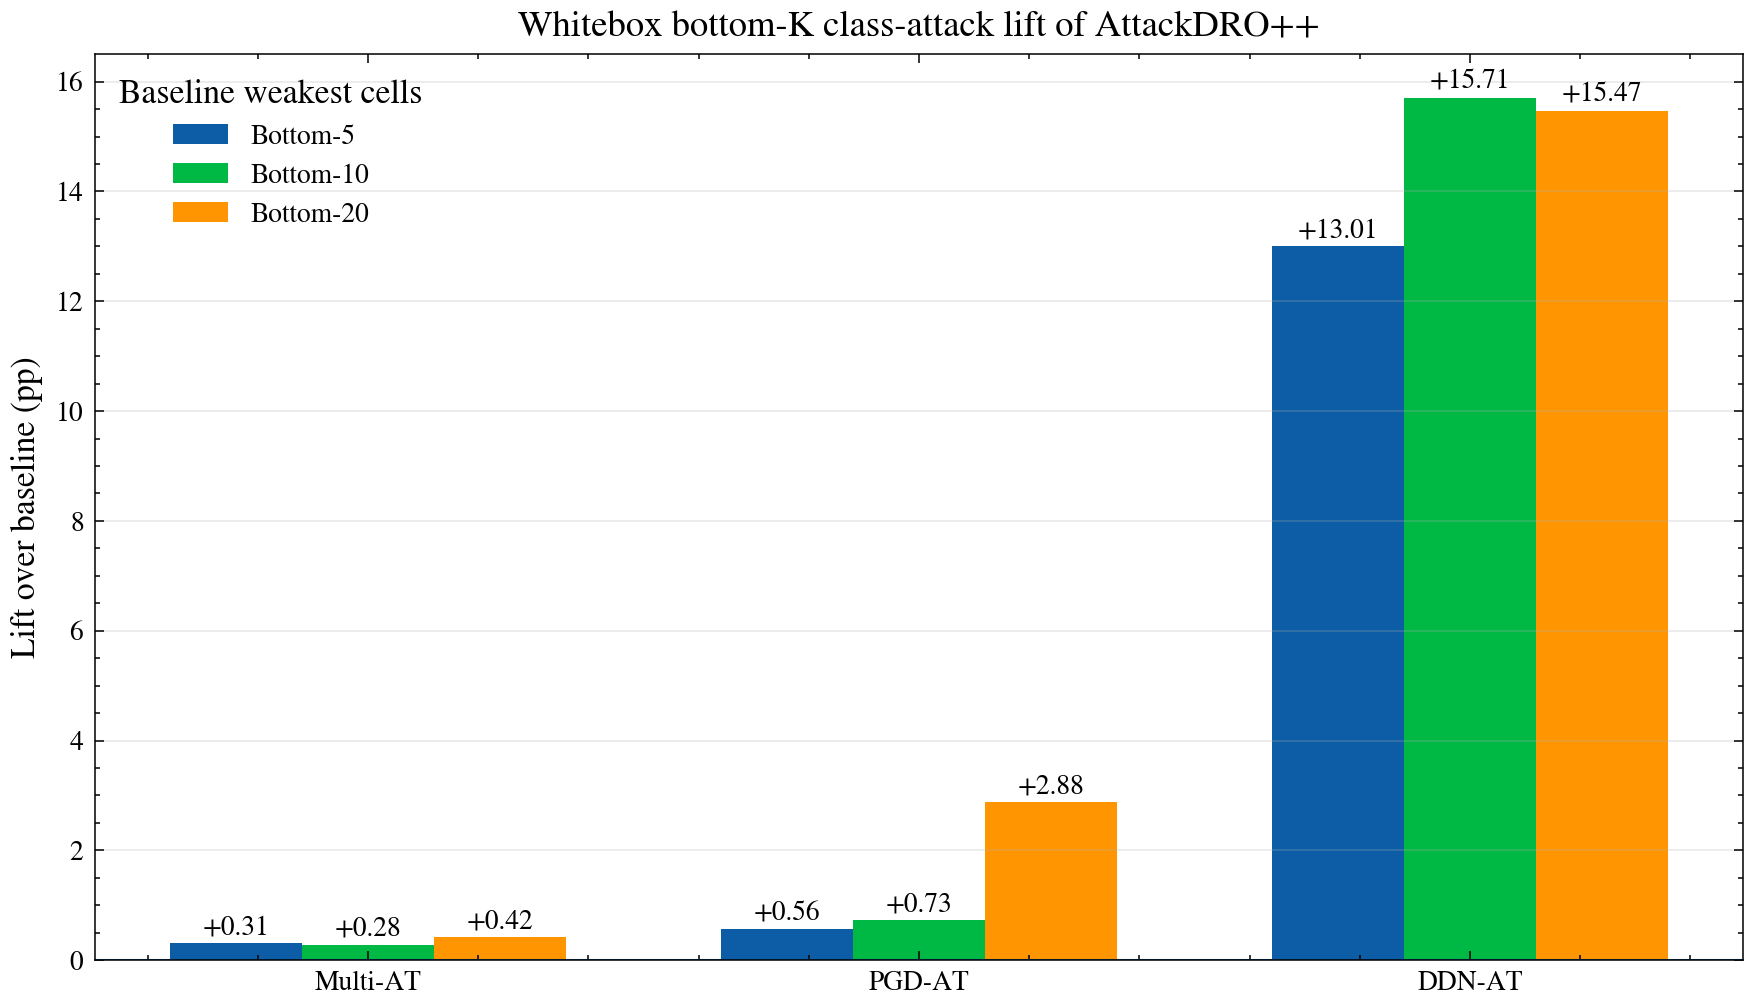
\includegraphics[width=0.64\linewidth]{figures/whitebox/whitebox_bottomk_lift_bar_n5.png}
\caption{Weakest-\(K\) whitebox class--attack lift of AttackDRO++ over each
baseline. For each baseline, the weakest-\(K\) cells are the lowest-accuracy
class--attack cells of that baseline; bars report AttackDRO++ minus the
baseline on those same cells.}
\label{fig:ch6_whitebox_bottomk_lift}
\end{figure}

The tail comparison is most pronounced against DDN-AT. Its weakest cells collapse
under \(\ell_\infty\)-oriented attacks, with the bottom-10 cells averaging only
\(15.602\%\). AttackDRO++ raises these same cells by \(+15.710\) pp, explaining
why it achieves a much more balanced whitebox profile than the \(\ell_2\)
specialist, even though DDN-AT remains competitive on several \(\ell_2\) cells.

Against PGD-AT, the lift is smaller but still positive: \(+0.726\) pp on the
bottom-10 cells. PGD-AT's weakest cells include several bounded \(\ell_2\)
attacks on difficult classes such as \textit{cat} and \textit{deer}; AttackDRO++
reduces many of these failures, indicating that multi-attack training and the
Cluster-DRO component help mitigate the cross-norm weakness of PGD-only training.

Overall, the weakest-cell analysis supports the aggregate conclusion from
Section~\ref{sec:ch6_whitebox}: AttackDRO++ gives a broad but modest refinement
over Multi-AT, substantially corrects the \(\ell_\infty\) tail weakness of
DDN-AT, and reduces the \(\ell_2\) tail weakness of PGD-AT.

The class-wise whitebox analysis shows where the aggregate gains appear and
which hard cells remain. It still evaluates attacks generated directly against
the target checkpoint, so it does not answer whether the same robustness pattern
holds when adversarial examples are crafted on a different model. The next
section therefore moves to the graybox transfer protocol from
Section~\ref{sec:ch5_graybox_protocol}.
